\documentclass{article}

\usepackage[utf8]{inputenc}
\usepackage{amsmath}
\usepackage{amsfonts}
\usepackage{algpseudocode}
\usepackage{graphicx}
\usepackage{float}
\usepackage{gensymb}

\usepackage[style=numeric, sorting=none]{biblatex}
\addbibresource{References.bib}
\title{A Comparison of Deep Q Networks}
\author{Dylan Trollope \\\small Supervised by Prof. CJ Watkins}
\date{2022}

\begin{document}

\maketitle

\section{Abstract}

Inspired by Google DeepMind's \textit{Playing Atari with Deep Reinforcement Learning}\cite{mnih2013atari}, this project examines how Deep Neural Networks can be used in conjunction with Q-Learning to solve Reinforcement Learning problems - a form of learning called Deep Q Learning. We present the challenges of applying Deep Neural Networks to traditional Q Learning problems and how these challenges are overcome. A base Deep Q network is presented in the CartPole environment and iteratively improved upon to demonstrate the effects of different architectures used to solve the problem presented by CartPole. The network takes as input the state information currently available to the agent and outputs the action which the network predicts to maximise the value function of the agent. A set of experiments is done to find the best parameters for the Deep Q Network and performance using these parameters is recorded. We observe the dynamics of the agent in this environment, to understand the relationship that exists between the exploration and exploitation of the agent compared to the values of states. We observe that mechanisms such Experience Replay and making use of a \textit{Target Network}, the agent is able to successfully learn where good states exist in order to solve the environment.

We also examine the effects of "reward engineering": incentivising the agent to stay in states that may be thought of as \textit{ideal} states - states if in which the agent continually remained, would solve the environment. 

Try to apply the same architecture to other environments to see how generalisable the network is. 


\newpage
\tableofcontents
\listoftables
\listoffigures
\newpage



\section{Introduction}

Reinforcement Learning (RL) is learning from interaction - a type of learning in which an agent (or learner) seeks to reach a goal state within an environment. Rather than being told which action to take, the agent discovers which action is best to take, given its current state in the environment, by maximising some reward signal or function. 

Recent advances in the field of Deep Learning have made it possible to extract high level features from high-dimensional input data, such as the creation of the convolutional neural network for image recognition and the transformer for speech recognition and language processing [references].

The fields of Deep Learning and Reinforcement Learning can be combined into a type of learning called Deep Reinforcement Learning, which has shown to give agents the ability to make decisions from large amounts of input data (such as a snapshot of an Atari game) in order to maximise their reward in order to reach a goal\cite{mnih2013atari}. 

In this report, several Deep Reinforcement Learning architectures, known as Deep Q Networks, will be implemented and compared in a number of Environments available in OpenAI's Gym library\cite{brockman2016openai}. The aim of these comparisons will be to experiment with and discuss the performance of these networks in different environments and understand why these differences might occur. 

\newpage

\section{Literature Review}

\subsection{Reinforcement Learning: An Introduction}

\textit{Reinforcement Learning: An Introduction}\cite{Sutton1998} introduces reinforcement learning as learning from experience and rewards. It frames learning problems through the lens of dynamical systems, specifically learning to control Markov Decision Processes (MDPs) that exist in incomplete and stochastic environments. For the purpose of this project, it is used to formalise the idea of reinforcement learning problems as series of MDPs that terminate under specific conditions. Furthermore, this book is used to introduce the ideas of goals, rewards, policies and (Q) value functions and how to calculate and optimise for these functions. We also use the book to examine dynamic programming in form of value iteration and how we can use its concepts as the foundation for allowing an agent to learn in an environment. Lastly, we take a look at off-policy Temporal Difference (TD) learning - specifically Q Learning, in which the learned Q function directly approximates the optimal action-value function, regardless of the followed policy. 


\subsection{Playing Atari with Deep Reinforcement Learning}

This paper\cite{mnih2013atari} is the main inspiration for this project. It presents a cutting-edge model that was generalised to be able to ply several Atari games to an expert level by combining the fields of Reinforcement Learning and Deep Learning, known as "Deep Reinforcement Learning." This paper discusses the challenges of applying Deep Learning to Reinforcement Learning, discusses the Convolutional Neural Network architecture used during the training process and importantly, draws attention to Experience Replay as the mechanism by which learning is enabled and optimised. It's also observed that a similar problem had been solved using similar ideas: \textit{TD-gammon}, an agent that learned to play backgammon using reinforcement learning and self-play (the act of learning to play a game by playing against yourself), was able to play the game to an expert level. Similarly to the work presented in this report, TD-gammon used a model-free reinforcement learning algorithm similar to Q Learning to achieve such high level play.

\subsection{Notes on Q Learning}

\textit{Notes on Q Learning}\cite{RLNotes} was used to consolidate my knowledge of Q Learning, specifically the maths underpinning the ideas of rewards, return, value functions and the how the Bellman equation can be used to understand when a policy is optimal. It also helped in understanding how Q Learning differs from other TD methods and importantly, noting that the agent need not be aware of transition probabilities or expected rewards given its current state. 

\section{Introduction to Reinforcement Learning}



\subsection{Components of Reinforcement Learning}

Besides the agent and environment, there are several components that make up a whole reinforcement learning problem\cite{Sutton1998}, namely: 

\begin{itemize}
    \item A Policy dictates the agent's decision-making process at any given time. A policy is roughly a function that maps perceived states in an environment to actions to be taken when in those states. Policies can range from simple functions or choosing a value from a table to more complex, computationally expensive functions that may include Neural Networks. In general a policy will, given a state, assign probabilities to the actions to take in that state. 
    
    \item A reward signal: At each time step, the environment sends the agent a reward for the action it has taken. The reward signal defines the goal of a reinforcement learning agent - the agent seeks to maximise the reward it accumulates over time.
    
    \item A value function: While the reward signal indicates what are \textit{good} actions to take in the short tern, the value function tells the agent which actions are most valuable in the long term. In RL, the value of a state estimates how much reward the agent will accumulate in the future, starting from that state. The value function takes into account the states that are most likely to follow the current state and the rewards available at those states. For example, tt is possible that a state yields a low immediate reward but offers a high value as the states that follow all yield high rewards. The reverse may also be true.
    
    Values may be seen as secondary to rewards, as without rewards there are no values to estimate but the function of the value is to achieve more reward. Yet, it is the value function that must be considered when deciding which action is best to take as this will maximise the reward the agent receives over the long run, and ultimately bring the agent closer to the goal state. It will become clear later then, that finding methods to accurately estimate the value function is crucial in succeeding in RL problems.
    
    \item Lastly, RL problems may be comprised of a model of the environment: This is used to mimic the environment the agent finds itself in and can be used to make inferences about how the environment will behave. This allows predictions to be made about the environment: given a state and an action, the model may be able to predict the next state and reward from that action. This allows the agent to \textit{plan} - the agent may be able to take a course of action made from these predictions rather than only estimating what the next best state may be.
    
\end{itemize}


\subsection{Markov Decision Process}

Markov Decision Processes (MDPs) can be used to formalise sequential decision making. 

Given a process is in a state $s$, the \textit{decision maker} within the process chooses an action $a$ that is available to it in state $s$. At the next time step, the process moves into the state, $s'$, as a result of action $a$ from the previous time step and also gives the decision maker a reward, $R_{a}(s, s')$, corresponding to its new state.

The probability that a process moves into state $s'$ is dependent on the action chosen at the previous state, and is given by the state transition function $P_{a}(s, s')$ - the current state depends on the previous state $s$ and the action $a$ taken in the previous state. 

Formally, an MDP can be defined as a 4-tuple $\langle S, A, P_a, R_a \rangle $, where: 

\begin{itemize}
    \item $S$ is the set of states - the state space
    
    \item $A$ is the set of actions - the action space, where $A_s$ is the set of actions available in state $s$.
    
    \item $P_{a}(s, s')$ is the probability that action $a$ in state $s$ will lead to state $s'$
    
    \item $R_{a}(s, s')$ is the reward received from after transitioning to state $s'$ from state $s$ after taking action $a$
\end{itemize}


\subsection{Interaction between Agent and Environment}

In RL, the agent (or \textit{learner}) is placed inside an environment, comprised of everything outside the agent. The agent selects varying actions to perform, which present new situations (or states) to the agent. Every action taken in an environment also produces a reward - a numerical value that the agent aims to maximise over time by the selecting the \textit{best} actions\cite{Sutton1998}. 

\begin{figure}
    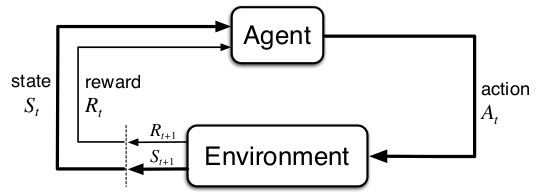
\includegraphics[scale=0.6]{images/Agent_Env_Interaction.png}
    \caption{The Agent-Environment Interaction Cycle\cite{Sutton1998}}
    \label{fig:ag_env_interaction}
\end{figure}


Formally, the agent and environment are in interaction with each other in a sequence of (discrete) time steps, $ 0 < t < T$. At each time step, $t$, the agent receives partial (or full) information about the environment's current state, $ S_t \in \mathcal{S}$ and selects an action $a$ at time $t$ from the complete action space, $A_t \in \mathcal{A}(s)$. 

At the next time step, $t+1$, the agent receives a numerical reward as a result of the action it took at the previous time step, $R_{t+1} \in \mathcal{R} \subset \mathbb{R}$ and is then in a new state, $S_{t+1}$. 

Together, the MDP and agent-environment interaction form a sequence as follows: 

$S_0, A_0, R_1, S_1, A_1, R_2, S_2, A_2, R_3 \cdots $


\subsubsection{Rewards and Return}

Over the Reinforcement Learning process, rewards are accumulated as the agent takes actions in sequential states of the environment. These rewards can be positive or negative. 

In Environments where rewards are positive, the agent most likely aims to maximise these rewards. In Environments where the rewards are negative (also referred to as costs), the agent may seek to minimise these rewards (costs)\cite{RLNotes}.

In an MDP, the agent seeks to maximise its \textbf{return}. The return may be thought of as an \textit{average reward} over a long run of decisions. The maximisation of the return will be considered the \textit{goal} of the agent, which is a distinct feature of reinforcement learning, compared to other forms of learning.

Given that an agent receives rewards at sequential time steps, 

$R_{t+1}, R_{t+2}, R_{t+3}, R_{t+4}, \cdots, R_T$, the simplest return of the agent can be calculated as: 

\begin{equation} \label{eq:1}
\rho_{t} = R_{t+1} + R_{t+2} + R_{t+3} + R_{t+4} + \cdots + R_T
\end{equation}

This return function is used when the RL problem is episodic in nature as it expects a final state at time $T$, which is the terminal state.

As can be seen from above, the return function is linear - immediate rewards and future rewards are \textit{weighted} equivalently, there is no incentive for the agent to take actions that would maximise reward over the long run or the short run, which for certain environments may be desirable. 

By introducing a discount factor into the return function, the agent can account for maximising more immediate or future rewards\cite{RLNotes}: 

\begin{equation} \label{eq:2}
\rho_{t} = R_{t+1} + \gamma R_{t+2} +  \gamma^2 R_{t+3} + \gamma^3 R_{t+4}  + ... = \sum_{k=0}^{\infty} \gamma ^k R_{t+k+1}
\end{equation}

where $0 \leq \gamma \leq 1$ is the discount rate and determines the value of future rewards that the agent receives. If the agent receives a reward $k$ time steps in the future, it is only worth $\gamma^{k-1}$ times what it would be worth if it were received immediately.

With $\gamma$ close to 0, the agent is very short-sighted and only concerned with maximising immediate rewards - it will choose an action $A_t$ to only maximise $R_{t+1}$.

With $\gamma$ approaching 1, the return function takes future rewards into account more significantly and the agent is more farsighted. 

Using equation (\ref{eq:2}) above, it can be shown how return functions at successive time steps are related\cite{Sutton1998}\cite{RLNotes}:

\begin{align}
\rho_t &= R_{t+1} + \gamma R_{t+2} +  \gamma^2R_{t+3} + \gamma^3R_{t+4} + ... \nonumber \\
     &= R_{t+1} + \gamma (R_{t+2} + \gamma R_{t+3} + \gamma^2 R_{t+4} + ... )  \nonumber \\
     &= R_{t+1} + \gamma \rho_{t+1} 
\end{align}

$\gamma$ is used to define a \textit{soft} time horizon (Watkins, 2021). The greater the amount of time steps away from the current state, the less the return calculated from those time steps


\subsection{Policy and the Value Function}

\subsubsection{Policy}

Most RL algorithms are concerned with estimating a value function - a function that estimates how \textit{good} it is for an agent to be in a state or how \textit{good} it is to perform a given action in a given state. A state is \textit{good} if the expected reward, or more specifically, expected return from that state to the terminal state is maximised\cite{Sutton1998}. Because future expected return is dependent on the sequence of actions taken by the agent in consecutive time steps, the value function is defined in terms of the behaviour of the agent, called a \textbf{policy}.

Formally a \textbf{policy} is a function that maps states to the probability of selecting the possible actions in those states and is denoted by $\pi$. In general, RL algorithms will attempt to find the optimal policy. An optimal policy is the policy that will maximise the expected return, starting in any state.

If an agent is following policy $\pi$ at time $t$, then $\pi(a|s)$ is the probability that $A_t = a$ and $S_t = s$. The policy defines a probability distribution over $a \in A(s)$ for each $s \in S$. 

RL algorithms specify how the agent's behaviour changes as a result of its experience.

**Deterministic vs stochastic policies and policy space**

\subsubsection{Value Function}

The value function of a state $s$ under policy $\pi$, denoted $v_\pi(s)$, is the expected return from state $s$ to the terminal state under policy $\pi$.

From the perspective of an MDP, the value function can be defined as follows\cite{RLNotes}\cite{Sutton1998}: 

\begin{align}
    v_\pi(s) &= \mathbb{E}_\pi [\rho_t | S_t = s, \pi]  \nonumber\\
             &= \mathbb{E}_\pi \left[\sum_{k=0}^{\infty} \gamma ^k R_{t+k+1}| S_t = s, \pi\right]
\end{align}
for all $s \in \mathcal{S}$, where $\mathbb{E}_\pi$ denotes the expected value of return given the agent follows policy $\pi$ at any time step $t$. 

The function $v_\pi$ is known as the \textit{state-value function}.

As will be useful later, Equation (4) can be rearranged as follows\cite{UCBSlides}: 

\begin{align}
    v_\pi(s) = R(s, \pi(s)) + \gamma \mathbb{E}_{s' \sim P(s'|s, \pi(s))} \left[ v_\pi(s')\right]
\end{align}

where the first term in the equation is the immediate reward and the second term is the return gained from the successor states when starting at state $s$ and following policy $\pi$.

\subsubsection{Q Value}

It is also possible to define the \textit{action-value function} under policy $\pi$, which is the expected return starting from $s$, taking action $a$ then continuing under policy $\pi$\cite{RLNotes}\cite{Sutton1998}:

\begin{align}
    q_\pi(s, a) &= \mathbb{E}_\pi [\rho_t | S_t = s, A_t = a, \pi]  \nonumber\\
                &= \mathbb{E}_\pi \left[\sum_{k=0}^{\infty} \gamma ^k R_{t+k+1}| S_t = s, A_t = a, \pi\right]
\end{align}

It can be seen that the summation term above is the same as the summation term in value function in Equation (4) above, with the only difference being the action specified in the Q value calculation, i.e. The Q value can be written in terms of the value function. 

Just as Equation (4) can be rewritten in Equation (5), the equation in (6) above can be represented in the following way\cite{UCBSlides}: 

\begin{align}
    q_\pi(s,a) = R(s,a) + \gamma \mathbb{E}_{s' \sim P(s'|s, a)} \left[ v_\pi(s')\right]
\end{align}

The functions $v_\pi$ or $q_\pi$ can be estimated over time:

Given an agent follows policy $\pi$ and maintains an average of the expected return for each state encountered, then the average return for each state will converge to that state's value $v_\pi(s)$ as the number of times it is encountered approaches infinity\cite{RLNotes}.

If averages are kept for each unique action taken in each state, then the averages will also converge to the expected return of the action-value function, $q_\pi$\cite{Sutton1998}.

\subsection{Optimal Polices and Value Functions}

For finite MDPs, it is possible to define precisely what it means for a policy to be optimal\cite{Sutton1998}. 

Value functions define a partial ordering over policies. A Policy $\pi$ is defined to be equal to or better than a policy $\pi'$ if its expected return is greater than or equal to that of $\pi'$ for all states:

$\pi \geq \pi'$ if and only if $v_\pi(s) \geq v_{\pi'}(s)$ for all $s \in \mathcal{S}$.

The \textit{optimal policy} is that policy which is greater than or equal to all other policies - the optimal policy is not necessarily a unique policy and is denoted by $\pi_*$. 

The optimal state-value function can be formalised as: 

\begin{align}
    v_*(s) = \underset{\pi}{\text{max}}\ v_\pi(s)
\end{align}

for all $s \in \mathcal{S}$. \\


Similarly, the optimal action-value function, $q_*$ can be formalised as: 

\begin{align}
        q_*(s, a) = \underset{\pi}{\text{max}}\ q_\pi(s, a)
\end{align}

for all $s \in \mathcal{S}$ and $a \in \mathcal{A}(s)$


\subsection{Optimality and the Bellman Equation}

A key problem to consider is exactly \textit{how} to know when a policy is optimal.

Given that the optimal policy $\pi_*$ is the policy that maximises $v_\pi(s)$ for every $s \in \mathcal{S}$, the optimal return function, also known as a Bellman equation can be defined as follows\cite{Sutton1998}:

\begin{align}
    v_*(s) &= v_{\pi_*}(s) = \underset{a}{max}(R(s, a) + \gamma \mathbb{E}_{s' \sim P(s'|s, a)} \left[ v_{\pi_*}(s')\right]) \\
    \pi_*(s) &= \underset{a}{argmax}(R(s, a) + \gamma \mathbb{E}_{s' \sim P(s'|s, a)} \left[ v_{\pi_*}(s')\right]) 
\end{align}



It is possible to define the optimal value function and optimal policy in terms of the optimal $q$ value:

From Equation (5) and Equation (10), it can be derived that:
\begin{align}
    v_* (s) = \underset{a}{max} (q_*(s, a))
\end{align}


and also from Equation (7) and (11),

\begin{align}
    \pi_*(s) = \underset{a}{argmax}(q_*(s,a))
\end{align}

These equations, known as Bellman equations, must hold for every state of the RL problem and give the conditions for a policy and its associated value function to be optimal. 

\newpage

\section{Q Learning}

Now that it has been underlined that it is possible to know that a policy is optimal, \textit{Q Learning} (Watkins, 1989) is introduced as a method to calculate the optimal Q Values and subsequently the optimal policy for an RL problem\cite{Watkins:89}. As will be shown later, Q Learning will be the main algorithm built upon to perform Deep Reinforcement learning. 

Q Learning is a model-free RL algorithm that is used to learn the \textit{Q Value} of an action in a particular state. It is a model-free algorithm in the sense that:

\begin{itemize}
    \item the algorithm does not need to have a model of the environment to learn the best action to take in a given state, and 
    
    \item the algorithm can learn Q Values without knowing what the next state is, what the expected return of the subsequent states will be or what the transition probabilities from any state $s$ to $s'$ will be. 
\end{itemize}

It may seem intuitive that state transition probabilities need to be learned but this is not the case. Using Q-Learning it is possible for the agent to learn an optimal policy without ever learning state transition probabilities or expected rewards from states\cite{RLNotes}.

\subsection{Initial Setup}

The only data structure required to perform Q Learning is a table to store estimated Q values for every state and every action which is incrementally updated to approach the optimal policy.

For every state-action pair there is a $Q(s,a)$ value.

\subsection{Experience}

Q-Learning relies on episodes of experience to learn the optimal policy. 

An experience is a 4-tuple $ \langle s, a, s', r \rangle$
and describes the reward $r$ received when transitioning from state $s$ to $s'$ by taking action $a$.

\newpage

\subsection{Updates}

With the Q table initialised, Q values are updated until \textit{convergence}, as follows: 

\begin{algorithmic}
    \For{each episode} 
        \State Initialise s
        \For{each step of episode}
            \State Choose $a$ from $s$ using policy from Q
            \State Take action $a$ in $s$ and observe $r$ and $s'$
            \State $Q(s,a) \gets (1 - \alpha) Q(s,a) + \alpha (r + \gamma \underset{a'}{max}Q(s', a'))$
            \State $s \gets s'$
        \EndFor
        \State Until $s$ is terminal
    \EndFor
\end{algorithmic}

\subsection{Off Policy Learning}

Q Learning is \textbf{off policy} RL algorithm, in that it needs only the experience 4-tuple $ \langle s, a, s', r \rangle$ to learn the relevant $Q(s,a)$ values. The agent does not need sequential experiences in order to learn the optimal policy.

However, to converge to the optimal Q values, the algorithm does need to explore every combination of states and actions "repeatedly and thoroughly" (Watkins, 2021). It can be seen that Q-Learning requires very little awareness of the environment it is in and the algorithm is rather simple. All that is required is to repeatedly update the Q table using the algorithm above. 


\subsection{Converging to the Optimal Policy}

Q Learning uses approximate value iteration to find the optimal policy. This means that the learned policy "will become arbitrarily close to the optimal policy after an arbitrarily long period of time" (Daley, 2020). Using the Bellman equation as an iterative update (defined above), the value iteration algorithm converges to the optimal action-value function, $q_t \xrightarrow[]{} q_*$ as $t \xrightarrow[]{} \infty$. For this to occur, two conditions need to be met\cite{mnih2013atari}\cite{RLNotes}:

\begin{enumerate}
    \item The learning rate must approach 0. 
    
    \item Every state-action pair must be visited infinitely often. This is achieved as long as every action in a state has a non-zero probability of being selected. 
\end{enumerate}



\newpage

\subsection{Exploration vs Exploitation}

In RL, the agent tends to take actions which it has tried in the past and found successful in adding maximising its Q value. But, in order to discover these state-action pairs, the agent must take actions that it has not attempted before. This means that the agent needs to \textit{exploit} what it has already learned but it also needs to \textit{explore} new actions in previously unseen states in order to maximise the Q values. The problem that an RL agent faces is that if it were to only employ one strategy, it would almost certainly fall short of its goal, and so a balance between exploration and exploitation needs to be found in order to continually approach the optimal Q values and ultimately the optimal policy. 

\subsubsection{Trade-off}

When the agent explores, it can improve its current knowledge and gain better rewards in the long run if its exploration leads to the valuable states. However, when the agent exploits its current knowledge, it gets more immediate reward even if the behaviour of the agent is suboptimal in the long run. 

As the agent can not explore and exploit at the same time, it must make a trade-off between exploring the environment (improving its knowledge in the long run) and exploitation (using its current knowledge to gain reward in the short term). 

\subsubsection{The $\epsilon$-greedy Search Strategy}

It is essential to find the correct balance of exploration and exploitation. Initially the agent is unfamiliar with its environment and needs to explore its surrounding states. As the agent becomes more familiar with its environment and discovers valuable states, it needs to reach those states and explore its new frontier of unknown states. 

The $\epsilon$-greedy approach selects the action with the highest estimated value most of the time by exploiting what is already knows, but with a small probability $\epsilon$, the agent will explore the environment to observe valuable states that it has not yet discovered. 

As will be seen, in practice, the epsilon value is made to decay - the more the agent has discovered about the environment, the less likely it is to explore states that it has not seen before. This is because after a long period of learning, the agent will have encountered most states and does not need to explore as much as in the initial stages of learning.

\newpage


\section{From RL to Deep RL}

Deep Learning, a form of supervised machine learning, which uses neural networks to transform sets of (possibly high-dimensional) inputs to outputs, has shown significant progress in the fields of computer vision (such as YOLOv3 (Redmon, 2018)), natural language processing (such as BERT (Devlin et al., 2018)) and Bioinformatics in the form of AlphaFold (Jumper et al., 2021). 

\subsection{Applying Deep Learning to RL}

Using Deep Learning, agents can make decisions from large amounts of (unstructured) input data without being aware of the state space. It has been shown possible to play games like Atari Breakout to an expert level using Deep Reinforcement Learning (Mnih et al., 2013). Using a variant of Q-Learning, later described as a Deep Q Network, the model is able to learn policies directly from input data (4 consecutive frames of Breakout gameplay) using a Convolutional Neural Network and output a value function to predict future rewards. 


\subsection{Challenges to Consider when Applying Deep Learning to RL}

There are some challenges to consider in the application of Deep Neural Networks to problems that have been traditionally thought of as Reinforcement Learning Problems:

\begin{itemize}
    \item Firstly, Deep Learning (a type of \textit{supervised} learning) applications are able to find accurate, generalised models by using large volumes of hand-labelled training data. In comparison, RL algorithms tend to learn from a scalar reward function that can be \textit{noisy} and \textit{delayed} - delayed in the sense that the true reward for an action in a state may only be seen thousands of time steps after that action was taken. This type of delay does not exist in Deep Learning as, once the network is trained, there is an (almost) instant prediction between an input and its predicted label.
    
    \item Secondly, in deep learning, most networks are assumed to take as input, samples that are i.i.d (Independently and Identically Distributed). In comparison, RL encounters sequences of states that are highly correlated to each other - i.e. Getting to state $s'$ from $s$ may be completely dependent on taking action $a$. There may also be a distribution shift in the RL distribution as the algorithm learns new behaviours, which may present challenges to deep learning algorithms that assume the data distribution is fixed.
    
\end{itemize}

\newpage
\subsection{Neural Network as a Function Approximator}


When outlining the conditions needed for Q Learning to converge, it is stated that: 

$q_t \xrightarrow[]{} q_*$ as $t \xrightarrow[]{} \infty$. 


In practice however, it is impractical to use this approach as $q(s,a)$ is estimated for every sequence (episode) and so there is no generalisation between many sequences. To remedy this, a neural network with weights $\theta$ is introduced as a non-linear function approximation in order to estimate $q(s, a, \theta) \approx q_*(s,a)$. This network is known as a Q-Network (Mnih et al., 2013).  


\subsubsection{Training a Q-Network}

The Q-Network is trained by minimising a sequence of loss functions, $\mathcal{L}_i(\theta_i)$ that changes for every iteration,

\begin{align}
    \mathcal{L}_i(\theta_i) = \mathbb{E}_{s,a \sim p(s,a)} \left[ (y_i - q(s,a, \theta_i))^2 \right]
\end{align}

where 

\begin{align}
    y_i = \mathbb{E}_{s' \sim \mathcal{S}} \left[r + \gamma \underset{a'}{\text{max}}\ q(s', a', \theta_{i-1})|s,a \right]    
\end{align}

is the target for iteration $i$ and $p(s,a)$ is the probability distribution over sequences of states and actions, also known as the \textit{behaviour distribution}. The parameters of the previous iteration $\theta_{i-1}$ are kept fixed for the current iteration of the loss function $\mathcal{L}_i(\theta_i)$. It is important to note that, unlike in supervised learning where targets are fixed before learning, the targets for $\mathcal{L}_i(\theta_i)$ are dependent on the current network weights. 

Differentiating the loss function with respect to the weights, the gradient is as follows: 

\begin{align}
    \nabla_{\theta_i} \mathcal{L}_i (\theta_i) = \mathbb{E}_{s,a \sim p(s,a);s' \sim \mathcal{S}} \left[ (r + \gamma \underset{a'}{\text{max}}\ q(s', a', \theta_{i-1}) - q(s,a,\theta_i)) \nabla_{\theta_i}\ q(s,a,\theta_i) \right]
\end{align}

Because it is computationally expensive to compute the full expectations of the above equation, stochastic gradient descent can be used to optimise this loss function. If there are updates after every time step and the expectations are replaced by single samples from the behaviour distribution $p(s,a)$ and $\mathcal{S}$ respectively, we arrive at the Q-Learning algorithm (Mnih et al., 2013). 

\newpage 

\subsection{Model Free and Off-Policy}

Just as in Q-Learning, it is important to note that Deep Q Networks are \textit{Model Free} and  adopt \textit{Off-policy} learning.  

It is model-free in that it solves the RL problem directly by using samples from the state-space $\mathcal{S}$ without explicitly learning about the environment in which the agent is placed. It is off-policy in that it learns a \textit{greedy} strategy $a = \underset{a}{\text{max}}\ q(s,a,\theta)$ while ensuring adequate exploration of the state space\cite{RLNotes}\cite{mnih2013atari}. 

In practice, the behaviour distribution is selected by an $\epsilon$-greedy strategy that follows the strategy with probability 1 - $\epsilon$ and selects a random action with probability $\epsilon$\cite{mnih2013atari}.

\subsection{Experience Replay in Deep Q Networks}

Q-Learning makes use of episodes of experience, where the experience at time $t$ takes the form $e_t = \langle s, a, s', r \rangle$. 

In Deep Q Networks, we want to store these experiences $\mathcal{D} = e_1, e_2, ..., e_T$ in memory called an \textit{experience replay}. When training the Deep Q Network, the Q-Learning updates are applied to samples of the experience memory, $e \sim D$, drawn at random from the store of experiences, $\mathcal{D}$\cite{mnih2013atari}. 

Upon performing experience replay, the agent selects an action according to an $\epsilon$-greedy policy. A fixed-length history of experience is used in order to train the neural network. 

\subsubsection{Advantages of Using Randomly Sampled Experience Replay}

The Experience Replay approach described above provides some efficiencies during training\cite{mnih2013atari}: 

\begin{itemize}
    \item Each step of experience may be used in many weight updates, providing greater data efficiency
    
    \item As sequential experiences are highly correlated, using random samples ignores this correlation, reducing the variance in training over a long run
    
    \item Lastly, when learning \textit{on-policy}, the current parameters are highly influential on the next selected sample. For example, if the \textit{maximising} action is for the agent to move to the left, subsequent samples will be from the left hand side and likewise, if the maximising action moves the agent to the right, the next samples will be from the right. By using experience replay and off-policy learning, the behaviour distribution is averaged over many previous states and actions, avoiding big oscillations or divergence during learning\cite{mnih2013atari}. 
\end{itemize}

\newpage

\subsubsection{Drawbacks of Randomly Sampled Experience Replay}

Because of finite memory constraints, Experience Replay only stores the last $\mathcal{N}$ experience tuples, and tuples are sampled uniformly from $\mathcal{D}$. This means that all transitions between states are weighted of equal importance, when in practice there exist transitions that contribute substantially more to the long term return than other transitions\cite{mnih2013atari}.

\subsection{Deep Q-Learning Algorithm}

The full algorithm for Deep Q Learning is presented below

\begin{figure}[H]
    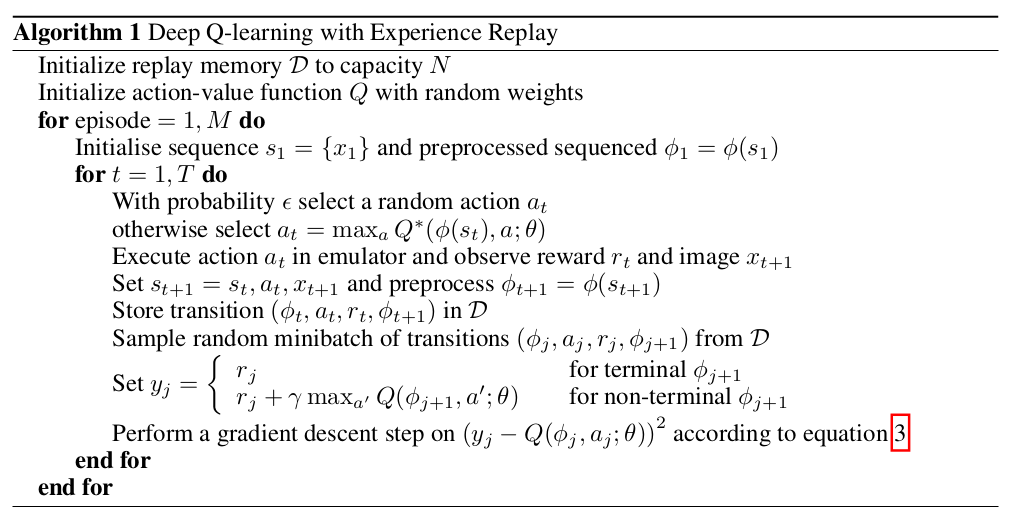
\includegraphics[scale=0.4]{images/DQN_DeepMind_Alg.png}    \centering

    \caption{Deep Q Network Algorithm \cite{mnih2013atari}}
    \label{fig:dqn_alg}
\end{figure}


\subsection{Deep Q-Learning Architecture}

The architecture consists of a fully connected Neural Network where:

\begin{itemize}
    \item The input layer, $i$ consists of $x$ nodes, where $x$ is the number of dimensions that the agent observes in the environment
    
    \item The second layer, $h_1$, consists of 64 fully connected nodes
    
    \item The third layer, $h_2$, consists of 128 fully connected nodes
    
    \item The output layer, $o$ has $y$ nodes, where $y$ is the number of actions available to the agent within the environment.
\end{itemize}




\section{The CartPole Environment}

The Environment in which the Deep Q Networks are tested is the CartPole Environment\cite{brockman2016openai}, which entails a pole balancing atop a cart which moves in the (frictionless) horizontal plane. The pole is attached to the cart by an unactuated joint. The goal of the environment is to balance the cart on the pole for as long as possible by moving the cart from side to side. The Environment ends when the Cart moves out of (horizontal) bounds (+/- 4.8 units from the centre of the environment) or if the pole falls more than 24 degrees from the centre. The Environment will also terminate if the reward reaches 500.  

The CartPole observation space is four-dimensional and is defined as follows: 

\begin{table}[H]
    \centering
    \begin{tabular}{|c|c|c|c|}
    \hline
    Index & Observation & Min & Max \\
    \hline
    0 & Cart Position & -4.8 & 4.8 \\ 
    1 & Cart Velocity & -Inf & Inf \\
    2 & Pole Angle & $-24^{\degree}$ & $24^{\degree}$\\
    3 & Pole Angular Velocity & -Inf & Inf \\
    \hline
    \end{tabular}
    \caption{Table of CartPole Observation Space}
    \label{tab:obs_space}
\end{table}




The action space is simple and two-dimensional: 

\begin{table}[H]
    \centering
    \begin{tabular}{|c|c|}
    \hline
    Action Number & Action  \\
    \hline
    0 & Push cart to the left \\
    1 & Push cart to the right \\
    \hline
    \end{tabular}    
    \caption{Table of CartPole Action Space}
    \label{tab:act_space}
\end{table}



\begin{figure}[H]
    \centering
    \includegraphics[scale=0.5]{images/cart_pole.jpeg}
    \caption{The CartPole Environment}
    \label{fig:cartpole}
\end{figure}

\newpage

To maximise the difference in architectures used, the following experimental parameters are used and kept constant between experiments: 

\begin{table}[H]
    \centering
    \begin{tabular}{c|c}
    \hline
    Variable & Value \\
    \hline
    episodes & 150  \\
    learning rate & 0.001 \\
    $\gamma$ & 0.9 \\
    $\epsilon$ & 0.3 \\
    decay & 0.99 \\
    \hline
    \end{tabular}
    \caption{Experimental Parameters}
    \label{tab:params}
\end{table}

\section{Experiments}

The experiments that follow were implemented using a host of Python libraries. The CartPole environment is accessed through the use of OpenAI's Gym library\cite{brockman2016openai}. The Neural Networks compared are created and trained using PyTorch\cite{NEURIPS2019_9015}. Lastly, the experiments were run in Jupyter Notebooks\cite{Kluyver2016jupyter} and plots rendered in Matplotlib\cite{Hunter:2007}. Throughout the experiments section, references will be made to snippets of the implementation of the experiments to bridge the understanding between Reinforcement Learning Theory and its Practical Implementation. The code used to implement many of the following experiments was adapted from several sources, namely \cite{mnih2013atari}\cite{ritakurban}.



\subsection{Random Strategy}

To create a base line for obtained reward and to later observe the effects of mechanisms such using a Neural Network as a function approximator and Experience Replay, we observe an agent trying to solve CartPole with a \textit{Random Strategy}. A random strategy means that the agent employs a policy where, at every time step, it takes a random action. It is expected that the agent fails completely to solve the environment, as no learning occurs and no information about prior states is used to inform its action in its current state. 


\begin{verbatim}
    for _ in range(episodes):
        state = env.reset()
        done = False
        total = 0
        while not done:
            action = env.action_space.sample()
            next_state, reward, done, _ = env.step(action)
            # env.render()
            total += reward
            if done:
                break
        reward_list.append(total)
\end{verbatim}

As can be seen from the implementation above, the action at every step is sampled randomly from the action space - there is no knowledge or experience considered when choosing an action. The format of this plot is inspired by \cite{ritakurban}.

\begin{figure}[H]
    \centering
    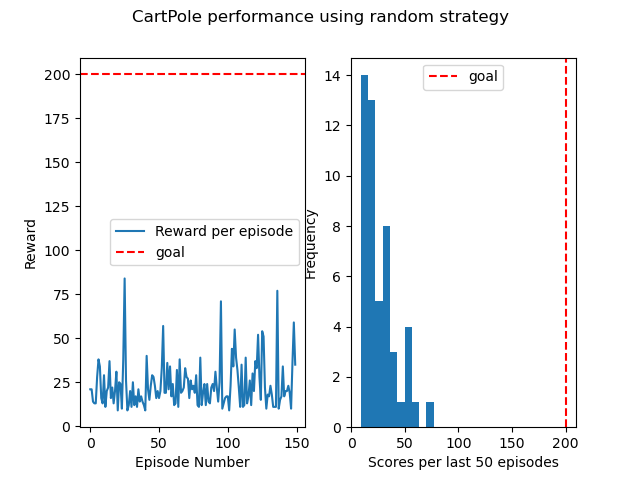
\includegraphics[scale=0.6]{images/Random.png}
    \caption{Reward vs Episode for the random strategy in the CartPole environment}
    \label{fig:cartpole_random}
\end{figure}

Using a reward score of 200 as the \textit{goal} reward, it can be seen that employing a random strategy is not effective in achieving the goal, as expected. The highest reward not being more than 100 points and so using a random strategy is not sufficient in achieving the goal state of the environment. 

As can be seen from the histogram on the right, the performance of the agent does not improve over time. Rewards over time do not approach the goal reward as the policy employed by the agent does not have any learning element.

Plotting the agent's performance over 3 runs - where a run is an agent retrained to solve the environment - produces the same observations: selecting a random action at every step does not allow the agent to solve the environment.

\begin{figure} [H]
    \centering
    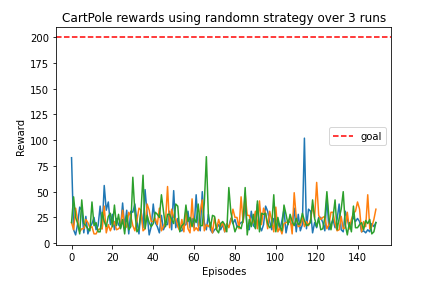
\includegraphics[scale=0.7]{images/Random3.png}
    \caption{CartPole Performance over 3 runs with Random Strategy}
    \label{fig:random_10}
\end{figure}

\subsection{Learning only from the Most Recent Action}

We now introduce the Deep Q Network as the mechanism by which the agent learns, explores and exploits its environment. Before introducing Experience Replay, we observe how well the agent performs by taking only the most recent action into account when performing its current action\footnote{The choice of optimiser, loss function, activation function and learning rate parameters will be motivated by later experiments}.

\subsubsection{The Network}

\begin{verbatim}
    SIZE = 64
    self.nn = nn.Sequential(
                torch.nn.Linear(state_dim, SIZE),
                nn.LeakyReLU(),
                nn.Linear(SIZE, SIZE * 2),
                nn.LeakyReLU(),
                nn.Linear(SIZE * 2, action_dim)
        )
        self.loss = nn.MSELoss()
        self.optimiser = torch.optim.Adam(self.nn.parameters(), lr)
\end{verbatim}

The snippet above defines the Neural Network used for Deep Q Learning. As stated before, it is a fully connected network that takes the observation space size as input, outputs Q Values for each action in the environment and has two hidden layers of size 64 and 128 respectively. 

% At each layer, Leaky ReLu is used as the activation function. We use Leaky ReLU 

\subsubsection{The Update Function}


The function below is used to update the Q Network given a training sample. It computes the loss given the current state's predicted Q value and the actual Q value produced by the network and then does a weight update using the ADAM Optimiser. 


\begin{verbatim}
        def update(self, state, y):
            y_pred = self.nn(torch.Tensor(state))
            loss = self.loss(y_pred, Variable(torch.Tensor(y)))
            self.optimiser.zero_grad()
            loss.backward()
            self.optimiser.step()
\end{verbatim}

\subsubsection{The Predict Function}

The predict function returns the Q values of the actions predicted by the network from the current state of the agent.

\begin{verbatim}
        def predict(self, state):
            with torch.no_grad():
                return self.nn(torch.Tensor(state))
\end{verbatim}


\subsubsection{Taking the Most Recent Action into Account}

In the training loop, we predict the Q value of the next state, then we assign the Q Value for each action given the estimate of Q values for the next state. Finally we update the model given the current state and the predicted Q value of the next state.

\begin{verbatim}
    q_values_next = model.predict(next_state)
    q_values[action] = reward + gamma * torch.max(q_values_next).item()
    model.update(state, q_values)
\end{verbatim}

\subsubsection{Performance Evaluation}

Plotting the performance of the agent over 150 episodes, the agent has been able to learn from the environment over time and slightly improve its performance - there is a clear upward trend in performance. However, it was only able to reach the goal score of 200 during one episode. 

Using a Deep Q Network to remember the most recent action improves the agent's performance but given the 150 episode constraint, it has not done very well.

\begin{figure}[H]
    \centering
    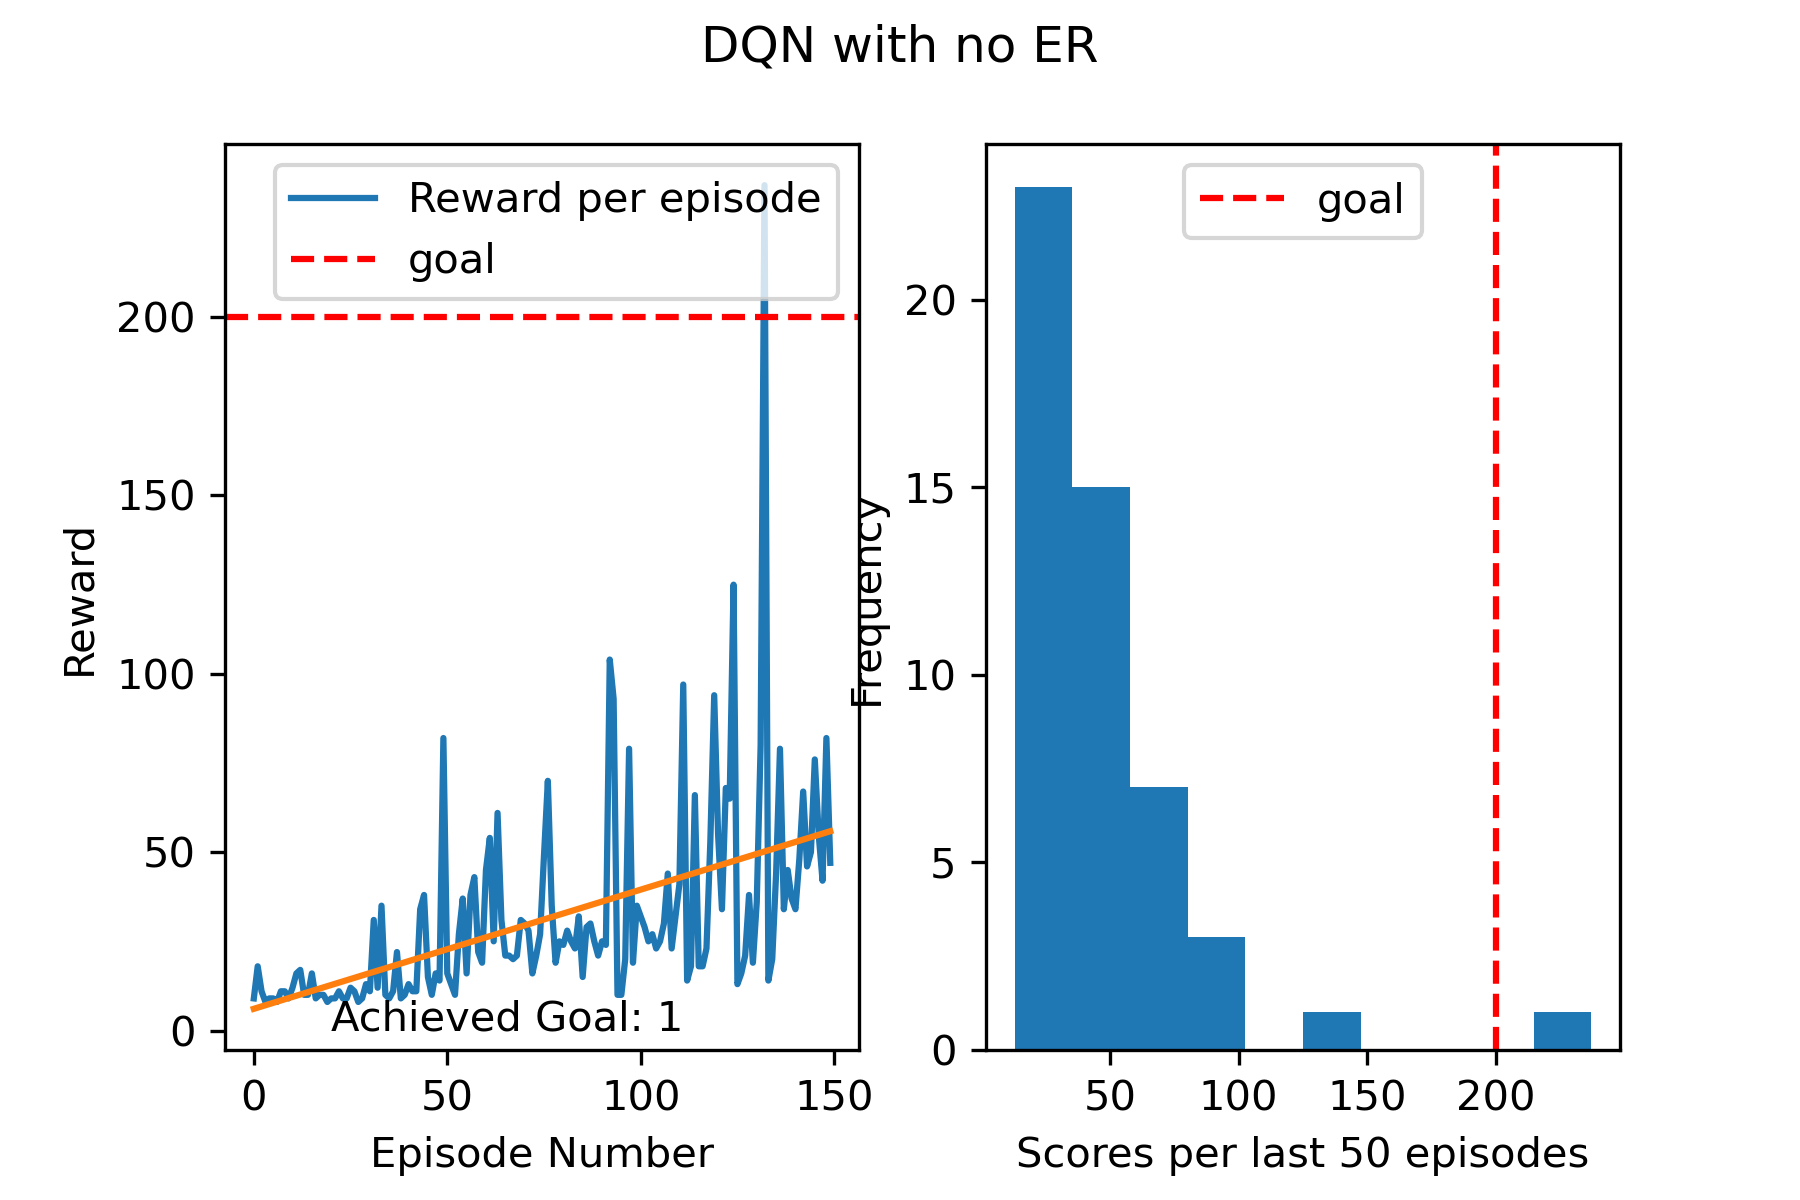
\includegraphics[scale=0.8]{images/SRHist.png}
    \caption{Deep Q Learning without Experience Replay in the CartPole environment}
    \label{fig:cartpole_memless}
\end{figure}


Evaluating the performance of the agent over 3 runs, where a \textit{run} is the retraining of the Deep Q Network, the same agent behaviour emerges: there is an upward trend in the agent's performance but it only reaches the goal state once in all three runs. 

\begin{figure}[H]
    \centering
    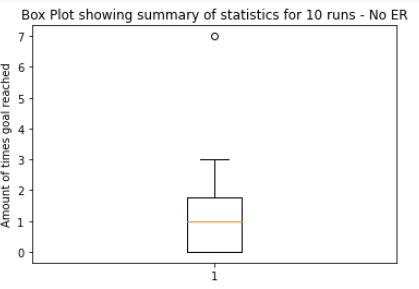
\includegraphics[scale=0.6]{images/SRBoxPlot.png}
    \caption{BoxPlot showing number of times agent reaches goal}
    \label{fig:SR_BoxPlot}
\end{figure}

\subsubsection{Loss Over Time}

As in most Deep Learning performance evaluations, it is useful to see the loss function over time. It should be expected that the loss (that is, the predicted Q value of the network vs the actual Q value produced by the agent) decreases over time, as the the network is trained to learn the characteristics of good, rewarding states. 

Because one episode is composed of many steps or actions, we take the average loss per step of each episode over 250 episodes. As the agent learns and exploits the environment more, the number of steps it takes greatly increases. Then calculating the loss as 

\begin{equation}
    \mathcal{L} = \frac{1}{n} \sum_{i=1}^{n} (y_i - \hat{y}_i)^2
\end{equation}
where $i$ is the current step and $n$ is the total number steps the agent takes that episode, the graph produced is as follows.

\begin{figure}[H]
    \centering
    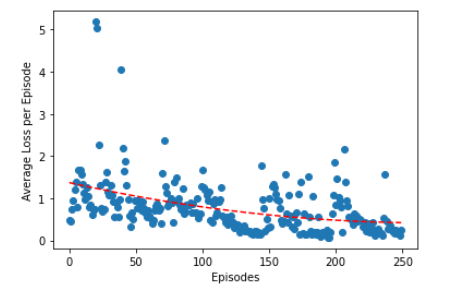
\includegraphics[scale=0.7]{images/SRLoss.png}
    \caption{Average loss over time for Deep Q Network with no Experience Replay}
    \label{fig:loss_sr}
\end{figure}

It can be seen that the loss decreases slightly over episodes, but there is a noticeable spread of losses over episodes, most extreme within the first 100 episodes. Noting that these episodes are where the value of $\epsilon$ is greatest, the high loss values can be attributed to the agent exploring and taking an action in a newfound state that lead to termination of the episode. 

As the model learns and starts exploiting its experience, instances of large loss values occur less frequently as the agent approaches having knowledge of the whole state space.

\subsubsection{Predicted vs Actual Q Values}

As well as understanding the behaviour of the loss function, it is interesting to see the Q value that the network predicts compared to the Q value that is learned or achieved by the agent.

To do this, we separate the agent's action space into \textit{left} and \textit{right} and see the Predicted vs Actual Q values of the network and agent, respectively.

\begin{figure}[H]
    \centering
    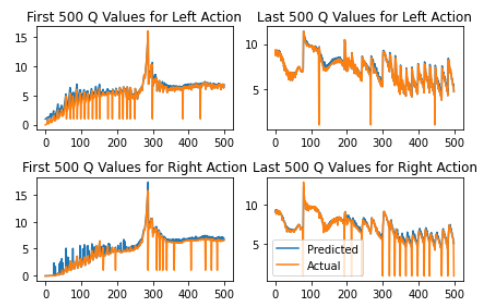
\includegraphics[scale=0.8]{images/QOverTime.png}
    \caption{Q Values in the first 500 and last 500 steps of training}
    \label{fig:SR_q_over_time}
\end{figure}

We can see that this slice of Q values approximates what is shown by the loss function plot above. The inaccuracy between the predicted and actual Q values is larger in the first 500 steps for both left and right actions, compared to the inaccuracy in the last 500 steps of the agent in the environment. By the end of training, the predicted Q value is able to approximate the actual Q value rather well. 

It is also interesting to note the difference in Q values between the different actions. For example, at the 300th step of training, the Actual Q value for taking the left action is zero. When observing the graph for taking the right action, the Q value is non-zero. At the same point in the graph for taking the right action, a non-zero Q value is learned for that state. This forms the basis of a useful sanity check: there are states in the environment that if the agent were to commit a certain action would cause the episode to terminate - a non-optimal outcome - in which the agent should expect a very small/zero Q value. 

There is however an obvious problem with the network - it has done very poorly in predicting where failed states that have Q values of zero exist. In general the network overestimates the Q value that is achieved (the predicted graph is always above the actual graph - never below it). 

\subsubsection{An Interesting Point about CartPole}

In many environments, Reinforcement Learning Specific and otherwise, an episode terminates when the goal state is reached. For example: 

\begin{itemize}
    \item In the classic RL environment, Mountain Car\cite{brockman2016openai}, the goal state as well as the termination state happen when the car reaches the flag atop the mountain.
    
    \item In the Atari game, Breakout, the game terminates when all the bricks have been destroyed (success).
\end{itemize}

CartPole is unlike these environments. CartPole terminates when it is unsuccessful (the cart moves off the screen in either direction or the pole falls over). For an agent to be successful in this environment then, it needs to avoid these terminal states (also referred to as \textit{doomed} states) for as long as possible in order to maximise its reward. The longer the agent can avoid the set of doomed states, the higher its reward value and the better its performance. 


\subsubsection{Missed Predictions}

The properties of the environment do begin to explain the network's poor performance in failed states. Because the environment terminates at a doomed state, the network is only able to make one parameter update before the agent encounters a valid state again. This means that the network is not well trained to predict doomed states compared to valid states - the distribution of encountered valid states compared to encountered doomed states is not equal. 

To remedy this, we introduce Experience Replay - it is possible that sampling from the agent's memory will aid in training the network to predict failed states as it may be exposed to more failed states from its memory.


\subsection{Where are the Good States?}

Although the CartPole observation space is four-dimensional, two of these dimensions can be used to give insight as to where the agent finds \textit{good} states. We take the Cart Position as the x-axis and the Angle of the Pole atop the Cart as the y-axis. Then, we a plot a heat map of Q values for every $(x,y)$ coordinate that the agent encounters. 

\subsubsection{Methodology}

To do this, it is necessary to discretise the continuous CartPole environment. By rounding the each dimension to two decimal places, we are able to generate a grid which is sufficient to draw some insight from the states that the agent encounters. 

We generate data by training the agent 100 times. We take the first 500 and last 500 steps of training for each run. This allows us to see the agent's initial and final perceptions of the environment. Of course, it is possible that the same \textit{(cart position, pole angle)} is visited multiple times. It is also important to note that the agent produces a Q value for both left and right actions in every state. 

So, the Q value calculated for a single $(x,y)$ location is the average Q value of all highest Q values produced by taking the best action in that state. 

Notably, not taking the other two dimensions into account presents a shortcoming in the experiment, but overall it is thought that the above chosen states are sufficient to "paint a picture" of what the agent learns from the environment. 

\begin{figure}[H]
    \hspace*{-3cm}
    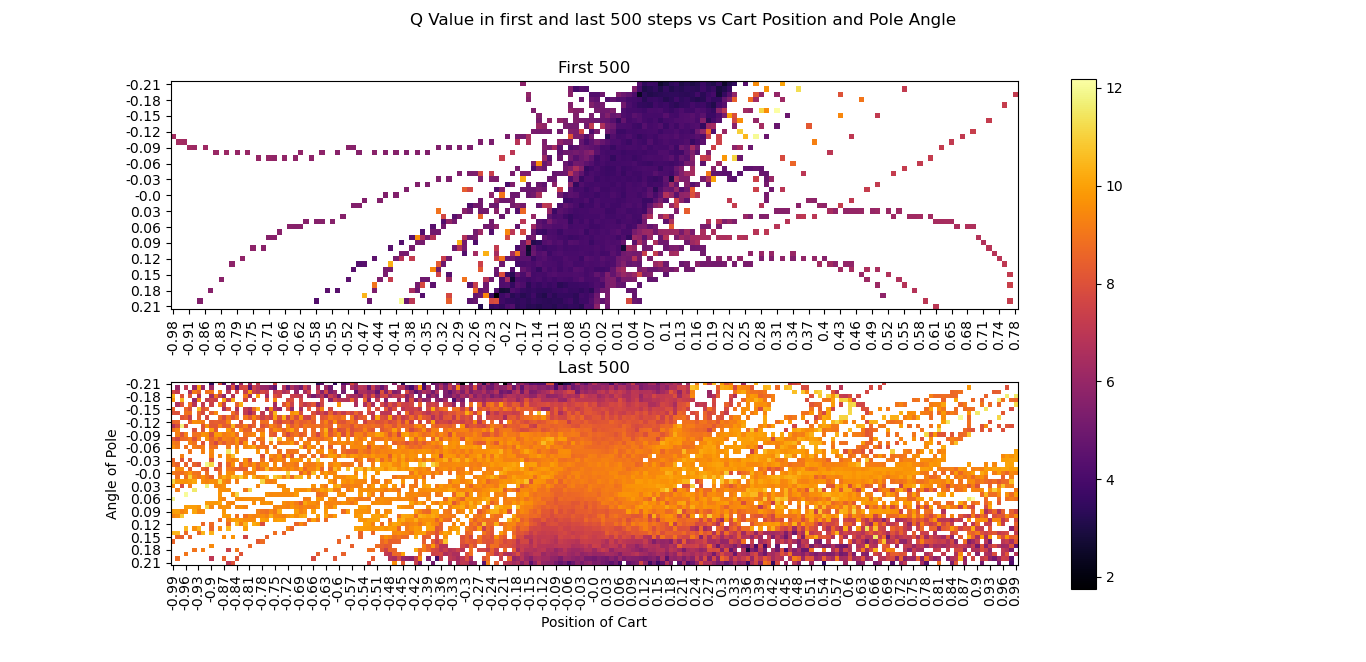
\includegraphics[scale=0.6]{images/SRQvsStates.png}
    \caption{Heat Map showing the Q values for encountered states}
    \label{fig:SRQvsStates}
\end{figure}

\newpage

\subsubsection{Observations}

Looking at the first 500 steps, some phenomena can be observed:

\begin{itemize}
    \item The majority of the encountered states occur when the cart is near the middle of the environment. This is due to the fact that the initial environment consists of the cart in the middle with the pole being pushed from the middle in a random direction.
    
    \item The majority of environments are terminated by the pole falling over rather than the cart moving out of bounds, seen by the mostly vertical bar of Q values. 
    
    \item The agent explores states away from the centre on several occasions, seen by the trail away from the central bar of Q values. These explorations are not immediately successful as the mostly purple trails show the Q value obtained at these states is low, when compared to the bottom graph. 
    
    \item The worst of the explored states (given by the deepest purple colour) is when the the pole is at its most angled. This observation makes sense in that, if the pole is at an extreme angle, it is very likely that the environment will soon terminate. 
    
\end{itemize}


The last 500 steps of training also give some interesting observations:

\begin{itemize}
    \item There is an emergent \textit{Z} shape that can be seen in the second graph. This is caused by the self-correction of the cart on the pole. More specifically, if the pole falls to the left (right) and the cart goes right (left) (upper right hand quadrant), the environment is likely to terminate relatively quickly, i.e. there won't be a long trail produced on the heat map by this episode.
    
    However if the pole falls to the left (right) and the cart moves to the left (right) to attempt "catching up" to the pole, a longer trail is produced on the heat map, although the states encountered in this type of episode are not seen to be very valuable, explaining the lower Q values (purple) at the horizontal edges of the Z shape.
    
    \item It can be seen that all four corners are much less populated than the centre - this makes sense as the agent has learned to mostly avoid the most extreme states (extreme cart position and pole angle).
    
    \item The most avoided and least valuable states are at the most extreme pole angles.
    
    \item It is more valuable for the agent to keep the pole upright than for the agent to stay in the centre of the environment.  

\end{itemize}


\newpage

\subsection{Introducing Experience Replay}

To see how effective Experience Replay is in the context of Deep Q Networks, the below experiment is conducted using a Deep Q Network with Experience Replay (ER). The implementation of ER is below: 

\subsubsection{The replay function}

\begin{verbatim}
    def replay(self, memory, size, gamma):
        if len(memory) >= size:
            states = []
            targets = []
            batch = random.sample(memory, size)

            for experience in batch:
                state, action, next_state, reward, done = experience
                states.append(state)
                q_vals = self.predict(state).tolist()
                if done:
                    q_vals[action] = reward
                else: 
                    q_vals_next = self.predict(next_state)
                    q_vals[action] = reward + gamma * torch.max(q_vals_next).item()
                targets.append(q_vals)
            self.update(states, targets)
\end{verbatim}

When there are sufficient samples in the agent's memory, it samples experiences in order to update the Q Network. For every experience, the network tries to predict the Q value of the next state, given the state of the experience, similarly to the network without ER. Then, we assign Q values to each action using the next state's predicted Q values. We then use the states in the agent's memory and its predicted Q values to do a model update.


\subsubsection{Performance Evaluation}

Compared to the Deep Q Network that only samples the most recent action, the Network with Experience Replay performs significantly better. The agent reaches the goal for the first time after approximately 50 episodes and goes on to reach the goal 72 times in total, almost half of the total episodes. 

It is interesting to note the main feature of the Reward vs Episode graph, in which the agent makes a clear improvement at approximately the 55th episode. From this episode onwards, the agent can be considered as having \textit{solved} the environment. However, from approximately episode 100, there is a decreasing trend in the agent's performance. The agent revisits states that allow it to achieve the goal but not necessarily continually improve its performance over episodes. 


\begin{figure}[H]
    \centering
    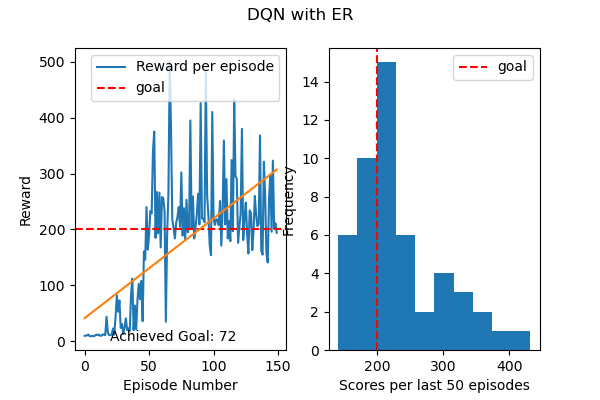
\includegraphics[scale=0.7]{images/ERHist.png}
    \caption{Deep Q Learning with Experience Replay for memory size $\mathcal{N}=10$}
    \label{fig:my_label}
\end{figure}

From observing the agent's behaviour, this is because of two reasons:

\begin{enumerate}
    \item When the agent (the cart in CartPole) has a "breakthrough" episode, the steep uptrend in the performance graph, it learns to keep the pole upright near the edge of the environment. This means that any small oscillations in the movement of the pole and subsequent cart reaction often means the cart leaves the environment, terminating the episode.
    
    \item The experiences sampled from the replay mechanism are experiences in which the agent had a low Q value predicted and so the model is (perhaps incorrectly) trained to take these actions that force the agent into lower performance scores. Later, we experiment with memory sizes to see what effect the amount of memory sampled has on the performance has on the agent. 
    
\end{enumerate}

We let the agent learn the environment over 10 unique runs to evaluate the average performance of the network in the CartPole environment. Below, a Box Plot is presented with the statistics for the amount of times the agent manages to reach the goal over 150 episodes with the default parameters. The agent manages to reach the goal an average of 73 times per 150 episodes, almost half of all episodes. 

\begin{figure}[H]
    \centering
    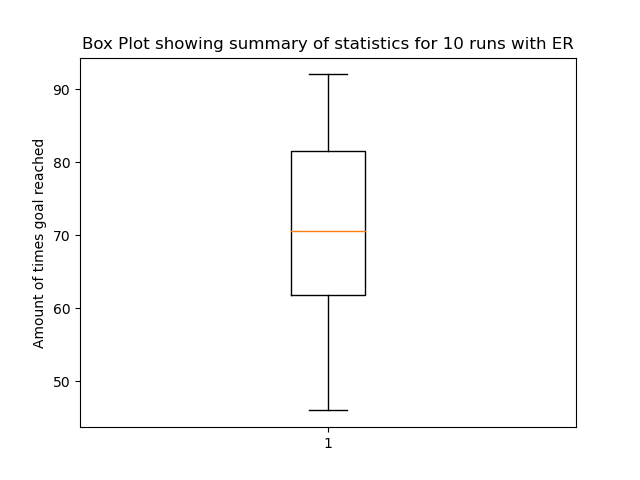
\includegraphics[scale=0.6]{images/ERBoxPlot.png}
    \caption{Box Plot for DQN with ER over 10 runs}
    \label{fig:ER13}
\end{figure}



From the above experiments, it is clear to see that the agent is capable of learning to solve the environment given it uses the Experience Replay mechanism to learn.

\subsubsection{Architecture Comparison: Conclusion}

The iterative improvement from random strategy to learning only from the most recent action to Experience Replay has shown improvement in the agent's ability to learn and the agent that uses Experience Replay has the most success in reaching the goal state in the environment.

The agent was unable to learn the environment using a Random Strategy which is expected. Learning only from the most recent action improved the agent's performance but still the agent was unable to regularly reach the goal state of the environment.

Using the Deep Q Network with Experience Replay, the agent was able to successfully learn how to solve the environment, able to reach the goal state in approximately half of all its runs.




\subsection{A Deep Dive into Deep Q Networks with ER}

\subsubsection{Loss over Time}

\begin{figure}[H]
    \centering
    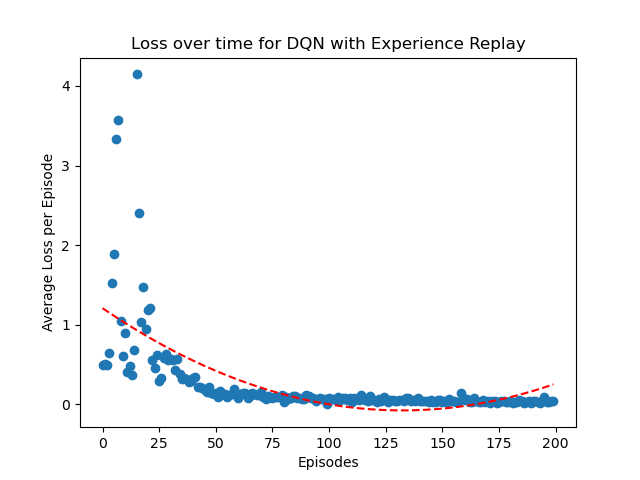
\includegraphics[scale=0.6]{images/ERLoss.png}
    \caption{Graph showing loss over time for DQN with Experience Replay}
    \label{fig:ER Loss}
\end{figure}

We now conduct some experiments to analyse the performance of the Deep Q Network with Experience Replay and observe how different parameters might affect the performance of the network and subsequently, the agent.

\subsubsection{Starting $\epsilon$ and Exploration vs Exploitation}

It is interesting to note how much exploration (choosing a new action from a given state) or exploitation (choosing actions that are known to produce high reward) the agent conducts and how this influences the performance of the agent. 

For values of epsilon in the range 0.3 to 0.7, we show how many times the agent reaches the goal state\footnote{The parameters for these experiments are the same as in \ref{tab:params}}

\begin{figure}[H]
    \centering
    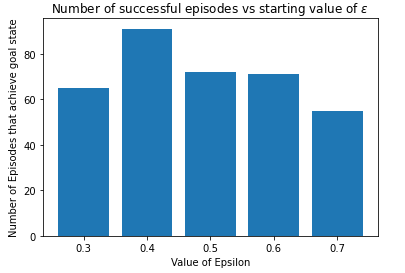
\includegraphics[scale=0.7]{images/SuccessesVsEpsilon.png}
    \caption{Exploration vs Exploitation}
    \label{fig:ExpExpSucc}
\end{figure}


\begin{table}[H]
    \centering
    \begin{tabular}{|c|c|}
    \hline
    Value of $\epsilon$ & \# of goal states reached \\
    \hline
    0.3 & 65 \\
    0.4 & 91 \\
    0.5 & 72 \\ 
    0.6 & 71 \\
    0.7 & 55 \\
    \hline
    \end{tabular}
    \caption{Amount of times the goal state was reached for different values of $\epsilon$}
    \label{tab:eps_vs_succ}
\end{table}




Although all values of $\epsilon$ produced reasonably good results, there is a clear difference in the choice of epsilon that performs best: 0.4. An $\epsilon$ of 0.4 is a \textit{sweet spot} for finding the balance of exploration to exploitation. A smaller value - in this case, 0.3 - possibly does not give the agent enough time to explore the environment before having to rely on its knowledge to find the best states. This means that the agent has stopped exploring the environment prematurely and not encountered states that are highly valuable. 

For $\epsilon$ values $> 0.4$, the inverse problem occurs: the agent explores the environment thoroughly but also finds states that are not considered very valuable. When these states are then sampled during the replay mechanism and the network trained on these states, the agent learns to find states that are sub-optimal.

Below, this is examined further. We plot the number of times the agent explored or exploited the environment for different values of $\epsilon$ for every step over every episode. The blue bars represent the amount of times explored while the red bars represent the amount of times the agent exploited the environment. 

As expected, the amount of exploration that occurred increases as the value of $\epsilon$ increases, seen by the increasing height of the blue bars. We expect that as the amount of exploration increases, the amount of exploitation decreases. From the graph, we observe that this is true for values 0.5 and above. However, when comparing $\epsilon = 0.3$ to $\epsilon = 0.4$, this trend is not followed. This is because for $\epsilon = 0.4$ and the nature of CartPole, the longer the agent can balance the pole, the more exploitation it can achieve.


\begin{figure}[H]
    \centering
    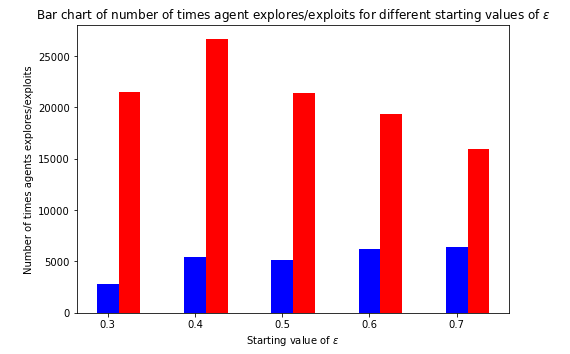
\includegraphics[scale=0.6]{images/ExploitExploreRatio1.png}
    \caption{Exploration vs Exploitation}
    \label{fig:Explore_Exploit}
\end{figure}

\begin{table}[H]
    \centering
    \begin{tabular}{|c||c|c|c|}
    \hline
    Value of $\epsilon$ & \# explored & \# exploited & Exploration/Exploitation (\%)\\
    \hline
    0.3 & 2848 & 21549 & 12/88 \\
    0.4 & 5466 & 26717 & 17/83 \\
    0.5 & 5175 & 21457 & 19/81 \\ 
    0.6 & 6262 & 19343 & 24/76 \\
    0.7 & 6438 & 16001 & 29/71 \\
    \hline
    \end{tabular}
    \caption{Ratio of exploration vs exploitation for different starting values of $\epsilon$}
    \label{tab:expexpratio}
\end{table}

The value $\epsilon = 0.4$ was then used when doing experiments with the remainder of the variables, as will be seen below.



\begin{figure}[H]
    \centering
    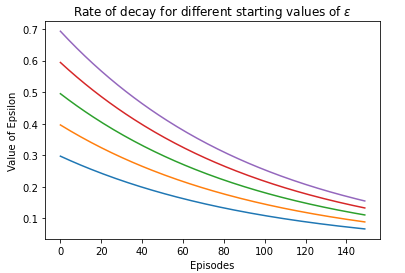
\includegraphics[scale=0.8]{images/EpsilonDecay.png}
    \caption{Exploration vs Exploitation}
    \label{fig:EpsilonDecay}
\end{figure}

\begin{figure}[H]
    \centering
    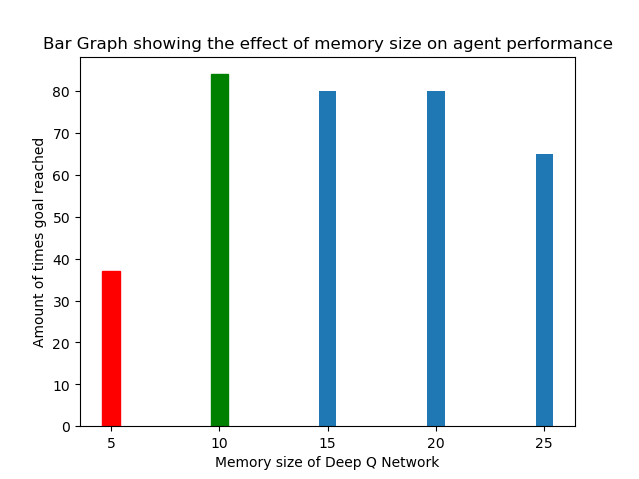
\includegraphics[scale=0.7]{images/mem_size_v_perf.png}
    \caption{Effect of Memory Size on Agent Performance}
    \label{fig:mem_size_vs_perf}
\end{figure}

\begin{figure}[H]
    \centering
    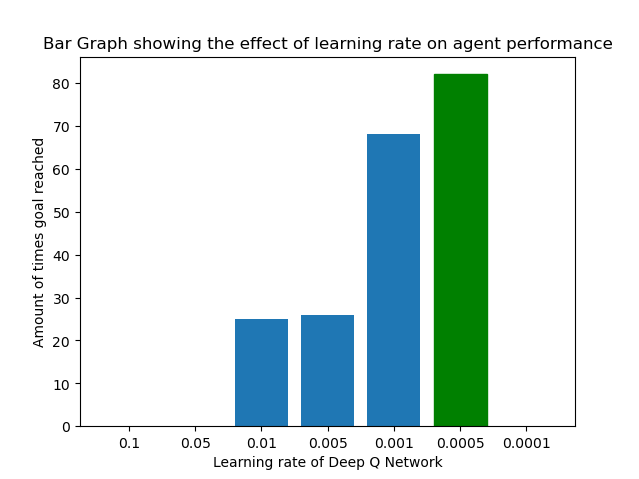
\includegraphics[scale=0.7]{images/lr_vs_perf.png}
    \caption{Effect of Learning Rate on Agent Performance}
    \label{fig:lr_vs_perf
    }
\end{figure}


\begin{figure}[H]
    \hspace*{-3cm}
    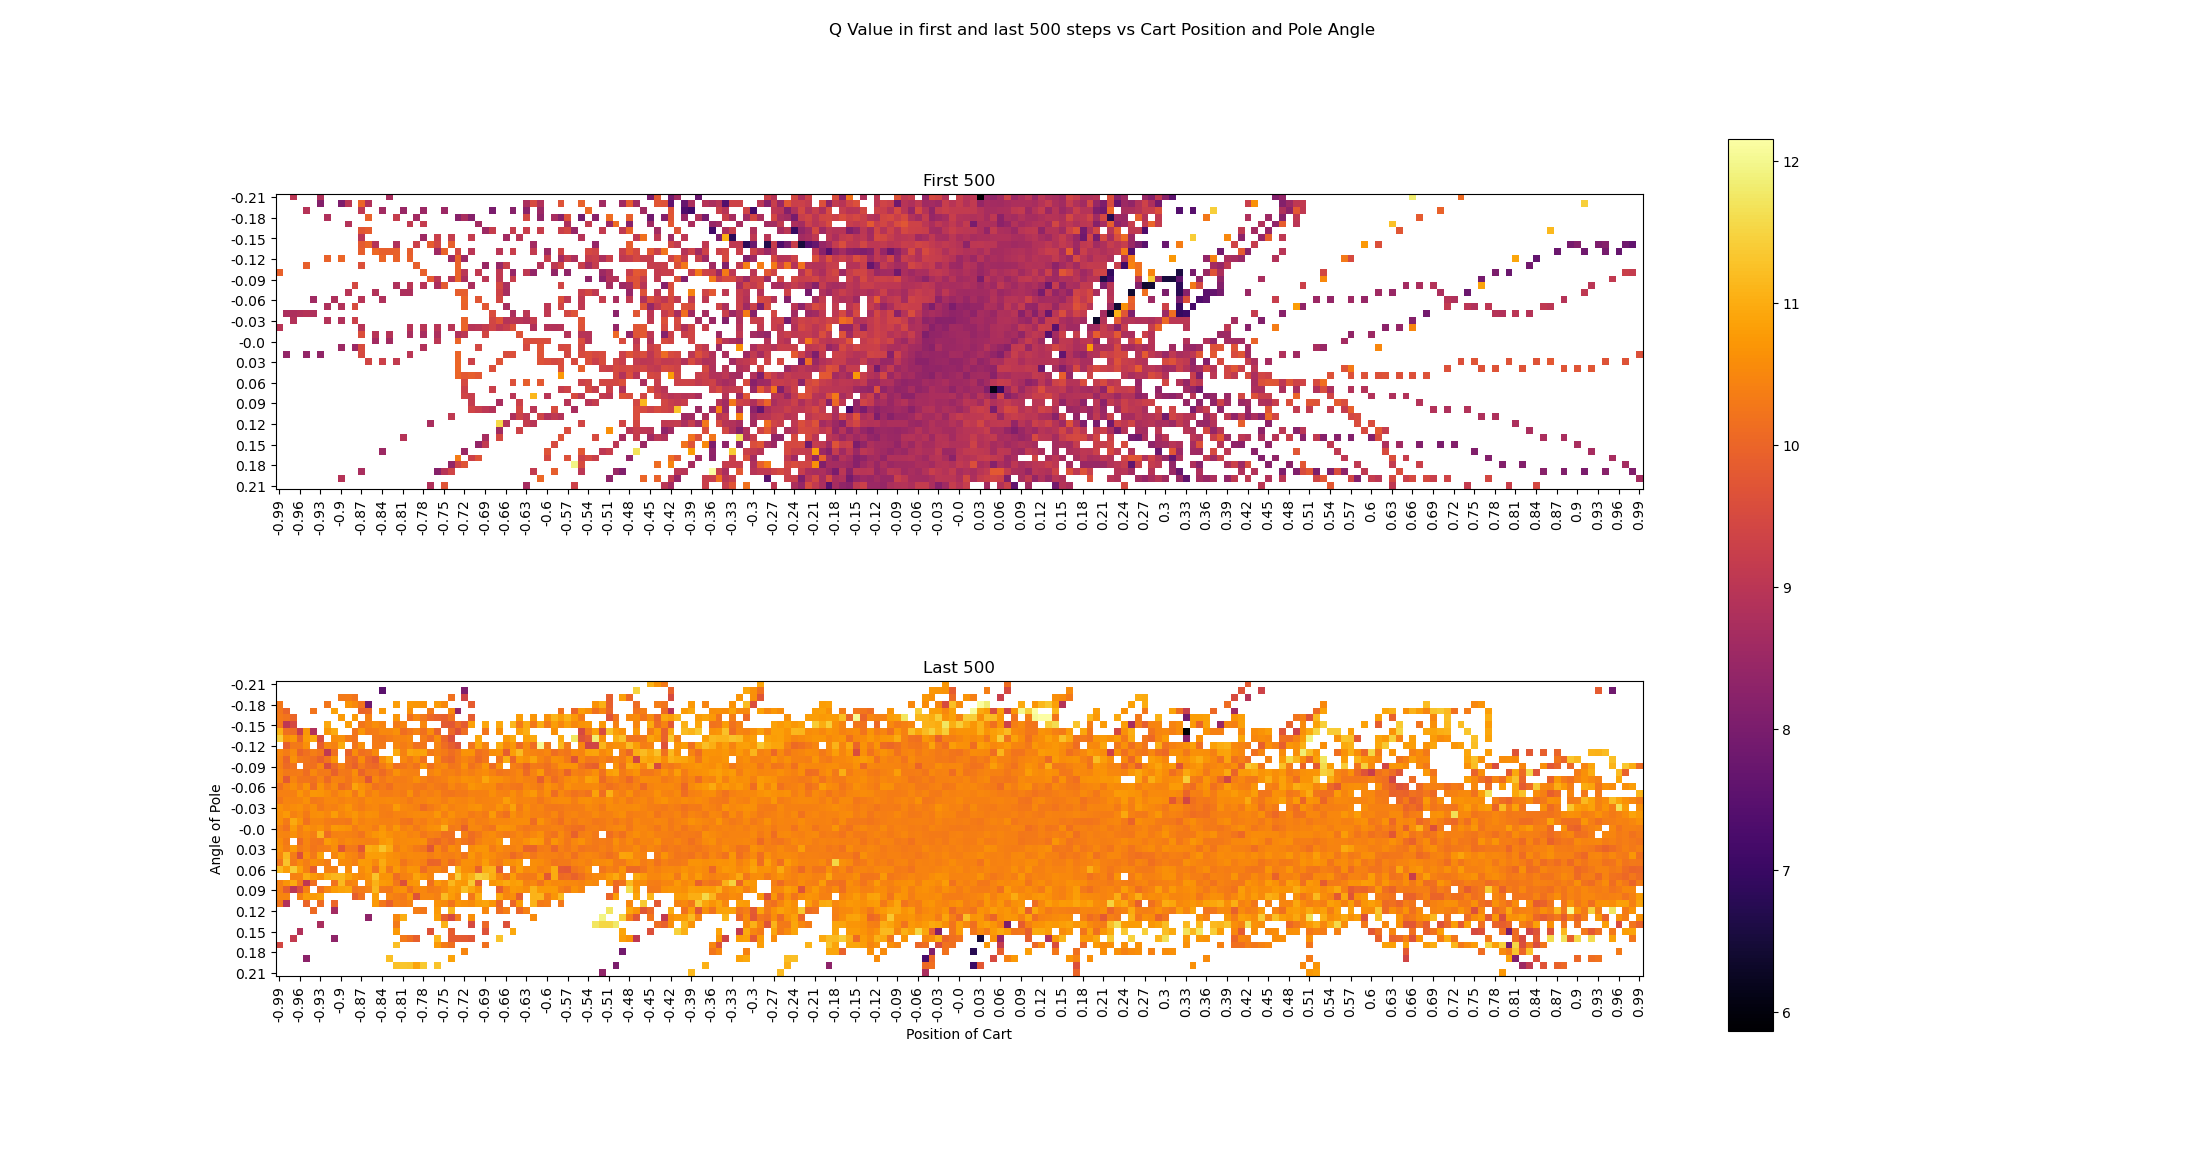
\includegraphics[scale=0.4]{images/QvsStatesER.png}
    \caption{Caption}
    \label{fig:my_label}
\end{figure}


\section{Conclusion}


\newpage 

\section{Self-Assessment}

\subsection{Positives}

\begin{itemize}

    \item In general, a good choice of libraries were used. In terms of interacting with the environment, OpenAI's Gym was a good choice. I was able to quickly get up and running to develop a proof of concept to see if it was a feasible library to use. The framework for action selection was modular enough to easily be able to plug in different mechanisms to assess how the agent would learn in the environment. Having significant experience in Python's NumPy and Matplotlib proved useful in conducting experiments efficiently. Having some PyTorch experience from this year's Deep Learning course proved very valuable. The Deep Q Network implemented in this project was straight forward and I did not have much bother in plugging it into the environment. 
    
    \item Because of the popularity of the original DeepMind paper\cite{mnih2013atari}, I was able to find a substantial amount of resources dedicated to the implementation of Deep Q Networks for several environments. Although the CartPole environment was not that popular amongst all possible environments, many of the same ideas\cite{ritakurban} applied when implementing and troubleshooting my program. 
    
    \item My framework for setting up experiments was set up early and worked well throughout the whole project. Having this framework it was simple to experiment with different values and variables and overall it was a section that was done well. 
    
    \item I conclude this project with a good understanding of Reinforcement Learning mechanisms, how we can frame these problems as a series of MDPs and why the breakthroughs in Deep Learning give such potential to solving other problems in the field of Deep Reinforcement Learning. I have also come to appreciate the challenge of attempting to integrate two different fields of learning into one and why the original work\cite{mnih2013atari} is considered with such high regard. 
    
\end{itemize}

\subsection{Negatives}

\begin{itemize}
    \item Initially the idea of the project was to do analysis of Deep Q Networks in many different environments. Because of obstacles experienced implementing different components of the program and due to time constraints, I settled on only exploring and experimenting with CartPole, as I felt that in-depth experiments and understanding in a singular environment was more valuable than broad, less informative experiments over many environments. 
    
    \item Briefly attempting to solve different environments with the same architecture was futile - because of how CartPole accumulates rewards and terminates compared to other environments. The closest was Lunar Lander I was unable to solve the environment successfully. 
    
    \item I underestimated how challenging it would be to implement a program by only reading the original research. Although many of the higher level concepts were easy to grasp, much of the underlying technicalities are vague and not discussed in the research. This meant that a lot of time was invested in small details of the implementation in order to obtain results.
    

\end{itemize}

\subsection{Improvements}

\begin{itemize}
    \item The most obvious improvement to be made to this project is to find the Deep Q model that generalises well to many different environments, just as in the DeepMind paper. Being able to experiment with multiple environments might have shed light on the components of the network that were most generalisable in order to achieve this.
    
    \item It would have been interesting to investigate whether a Convolutional Neural Network would have performed better than the Fully Connected Neural Network that was used instead.
    
    \item In terms of experiments, the plot of states vs Q values is difficult to read as the states were taken in slices, given that CartPole is 4-dimensional. It would have been interesting to see the same plots on a successful Deep Q Network implementation on a 2D environment like MountainCar.
    
\end{itemize}

\subsection{Looking Forward}

\begin{itemize}
    \item Upon completion of this project, I have gained the ability to reason about the integration of one field of learning with another. Looking ahead, I hope to be able to use this experience in the future - being able to reason about when it is possible to use the features of a particular domain and apply it to a separate domain and also understand when this is not possible.
    
    \item I have also gained experience in implementing and executing ideas from high level algorithms and ideas presented in cutting-edge research. As I look to a future in teaching, academia and hopefully research, I hope to harness these skills so that I am able to recreate future cutting edge ideas in the form of working software with the ability to experiment with these concepts and reach well-informed conclusions.
\end{itemize}


\newpage

\section{TODO}

\begin{itemize}
    \item Graph of predicted y vs actual y 
    \item Loss over time 
    \item Plot of Q values vs slices of states
    \item Memory size vs average goal achieved
    \item Optimisers: ADAM vs RMSProp vs ... 
    \item learning rate on agent performance
    \item Double DQN
    \item Replace average plots with box plots
\end{itemize}






\newpage
\section{Professional Issues}

\subsection{Explainable Artificial Intelligence}

Understanding why (or why not) machine learning models, specifically Deep Neural Networks, make the predictions they do is becoming an ever increasingly important question to answer as Artificial Intelligence emerges in the manufacturing, transport and medical sectors.

Historically, machine learning models have been opaque and difficult to understand \ref{}. Although there are examples of these models producing incredible results, like AlphaFold (which given the amino acid makeup of a protein can predict the 3D structure of the protein), the ability to do on-the-fly object detection and avoidance in the autonomous vehicle domain (Tesla and OpenPilot), and the ability to translate natural language in real-time (GPT-3(?)), there has up until very recently been a great focus on the results of these models and not the reasons or explanations for these results. 

\subsection{Black-box and White-box Models}

In the domain of Explainable Artificial Intelligence (XAI), there are two opposing approaches to creating machine learning models: \textit{black-box} and \textit{white-box} models. White box models provide results that are easy to understand for experts in their domain. On the other hand, black-box models are hard to explain and can usually not be understood by experts in that domain. 

In general, XAI models should aim to follow three principles, transparency, interpretability and explainability. A model is transparent if "the processes that extract model parameters from training data and generate labels from test data can be described and motivated by the approach designer." A model is interpretable if it is possible to present the basis for a model's decision making in a way that is easy for humans to understand. Although the exact definition for explainability is not yet agreed, it is considered the features of the interpretable domain that have lead to a model making a decision (classification or regression) for a specific example. 

If a model meets these three criteria, then it is possible to justify why the model makes a decision and consequently, it gives the ability to verify any decisions made on specific observations from the data. Meeting these criteria is also important as it is crucial for these novel systems to gain the trust of the public. A straightforward example is the autonomous car - being opaque or unable to justify why an autonomous vehicle makes a decision is a safety critical failure of the model with human life at stake. Although it is unreasonable to expect such systems make absolutely zero errors, it is important to consider and understand the basis for the decision making of these systems so that the designers are able to update their models to avoid the same errors in the future.
 
 
\subsection{Cooperation Between Humans and Agents}
 
Another domain where trust is paramount is the intersection between humans and machines powered by artificial intelligence and machine learning algorithms. It is crucial to have a formalised trust criteria so that when these systems are used in critical domains, like healthcare, the medical professional is able to trust the decision making process of the system to augment their own decision making process rather than doubt it.

\subsection{XAI in Unseen Data}

It is not uncommon for models to perform extremely well in the training phase but do poorly in the validation and test phase. For example, in a 2017 animal breed recognition system, the model learned that most pictures containing horses had a copyright symbol in the same corner of the image. This means that during training, the model learned that any image containing a copyright symbol contained a horse. During the validation and test phase however, the model performed very poorly as most observation contained the same copyright symbol. Using the idea of transparency in the context of XAI, this kind of "cheating" by the model should be understood and avoided (perhaps by using images that don't contain the copyright symbol, or by removing that corner of the image from each observation during training). Altogether, being able to understand and justify a model's decisions should also make it possible to improve the model during training and subsequent performance on unseen data. 


\subsection{Criticism of XAI}

There have been suggestions from researchers that the pursuit of XAI should be considered a secondary goal to the effectiveness of the actual AI systems and that encouraging the exclusive development of XAI systems broadly slows down the development and may limit the functionality of the decision making system. This critique is based upon empiric reasoning from evidence-based medicine that suggest AI technology can be clinically validated even if its internal function can not be fully understood. 

It has also been noted that XAI systems have been the primary focus of AI practitioners and not end users, with the opinion in the public over whether having XAI systems accompany machine learning models being fragmented. 

It is also important to note that there does exist a set of machine learning models that are inherently explainable, such as decision trees. In decision trees it is possible to see exactly which feature of the data is sampled and where, given that feature, an observation will lie in the decision tree. Researchers have noted that the use of these inherently explainable techniques are preferable to many XAI techniques, especially those in which a post-hoc (secondary) model is produced to explain the first model. 

It is also unclear whether XAI techniques will be able to remain effective a explaining why models make decisions the way they do as new AI and machine learning models tend to higher and higher complexities. 

\subsection{Conclusion}

It is clear that being able to reason about models is crucial when designing these systems, for the sake of public trust and for AI to be used in mainstream industries. It is important to understand and accept that there are also models in which XAI techniques are not yet feasible - this fact should also not be an obstruction to the ground breaking results that these models might produce, but also that it may be advantageous to treat any model with a certain amount of scepticism. 


 
 
 
 
 
 
 

 






















\newpage 
\printbibliography


\end{document}

